\chapter{COLLECTED MATERIALS AND MAKING OF}

% Toplamaya ve uretime ait fotograflar.
% Hepsi bir arada, defter nasıl dikilir, toplanan malzemeler.

\begin{figure}[h!]
  \centering
  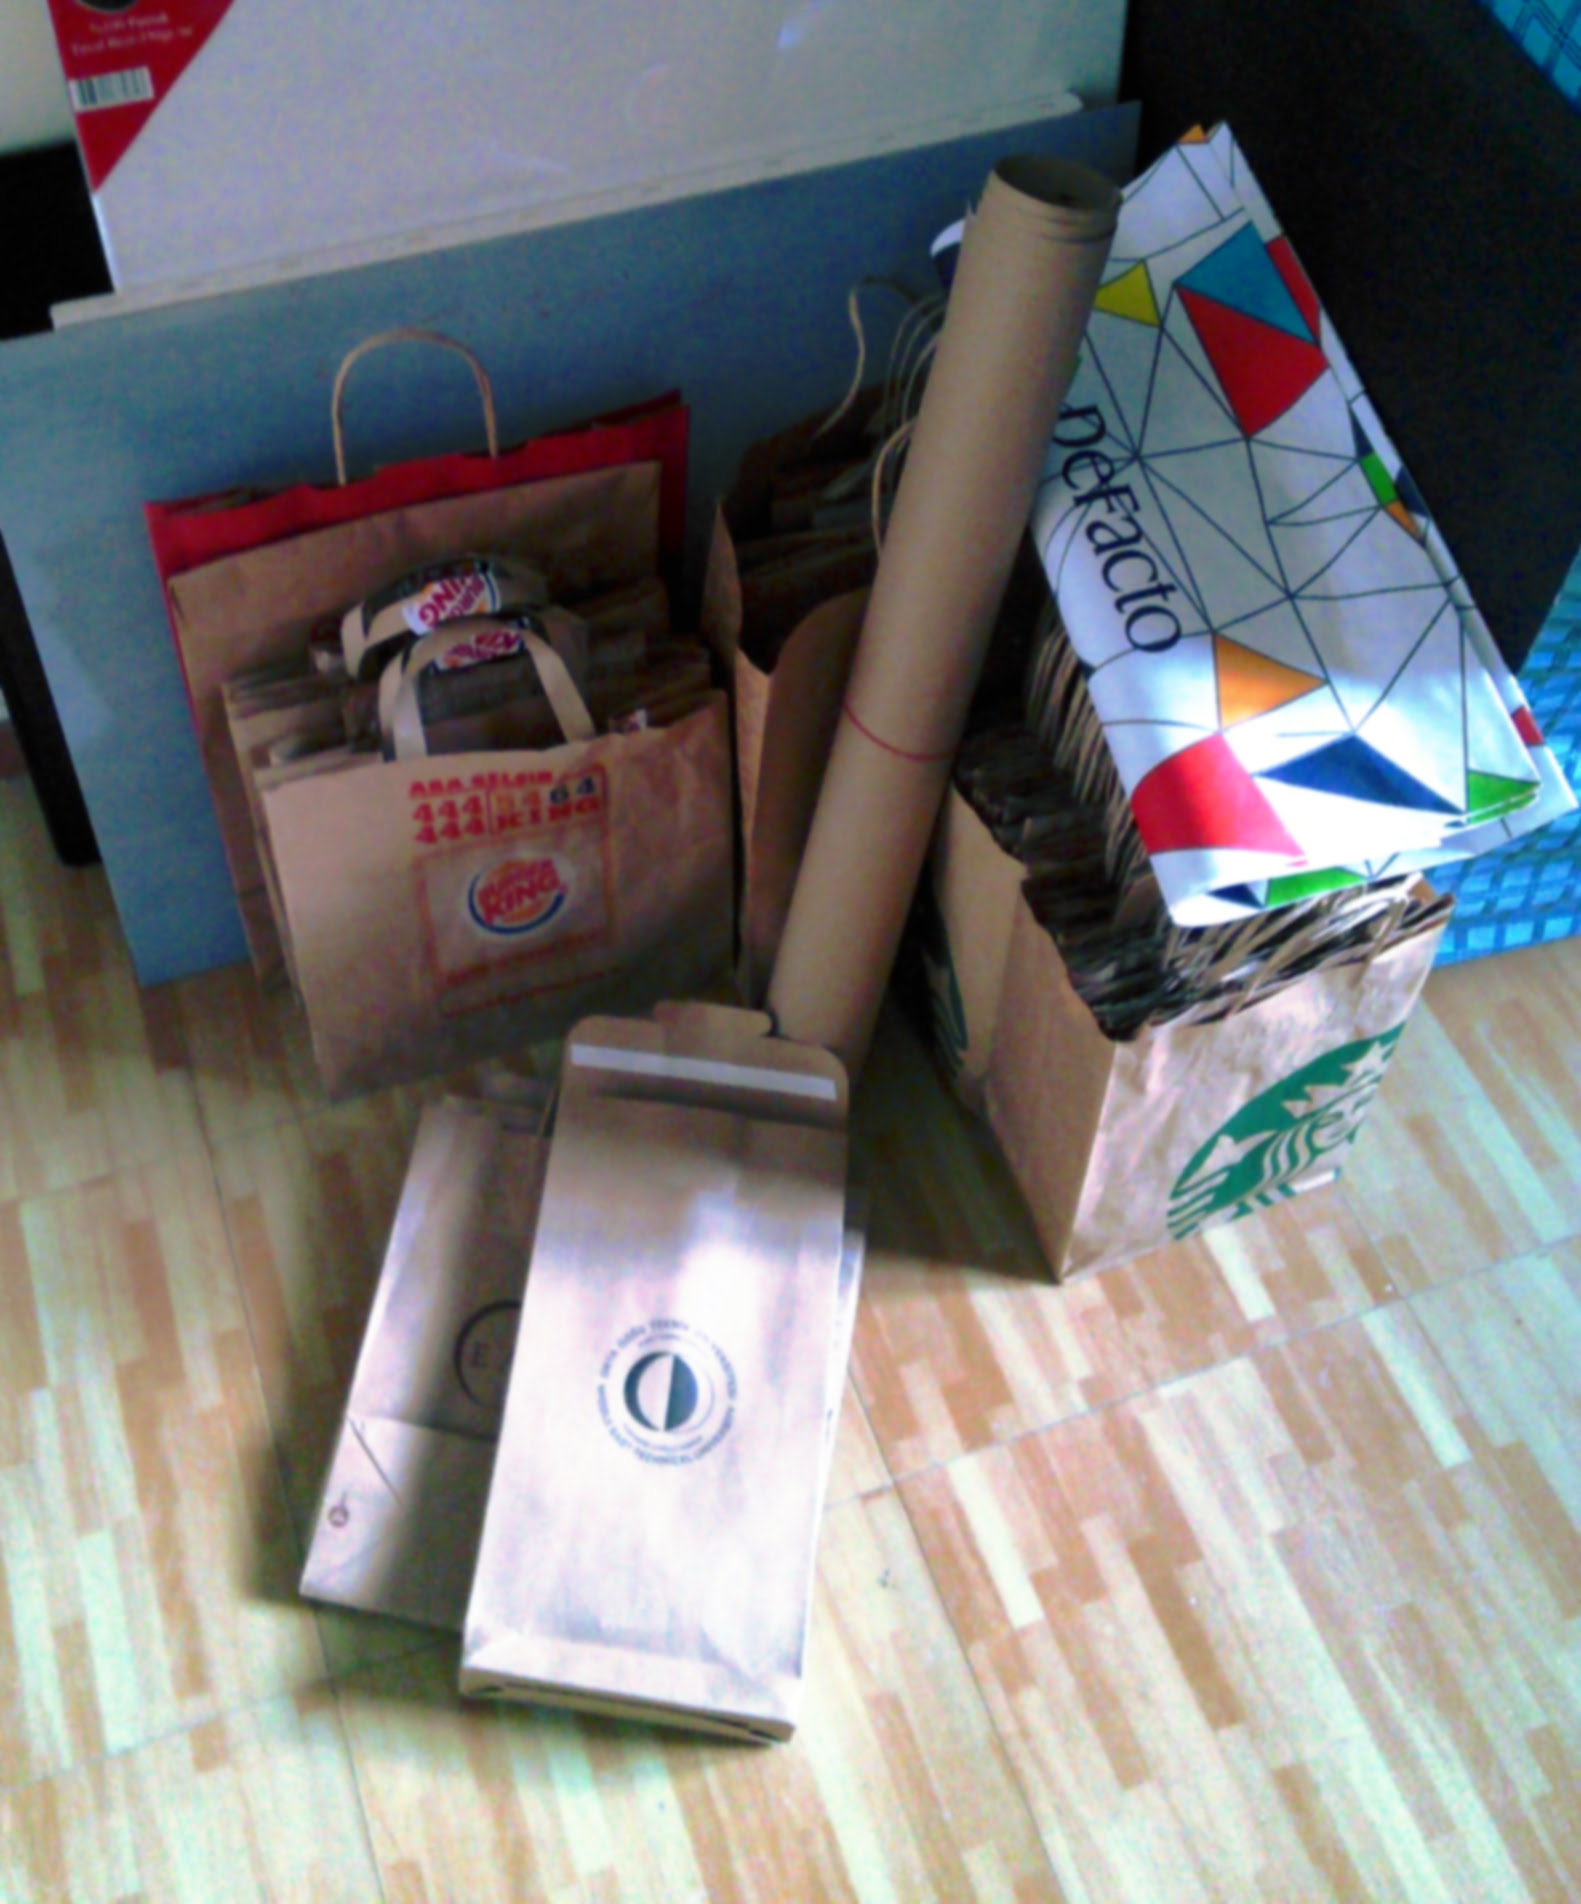
\includegraphics[height=10cm]{project_graphics/collected_all_together.jpg}
  \caption{Collected materials}
  \label{fig:CollectedAllTogether}
\end{figure}

\begin{figure}
    \centering
    \begin{subfigure}[t]{0.47\textwidth}
        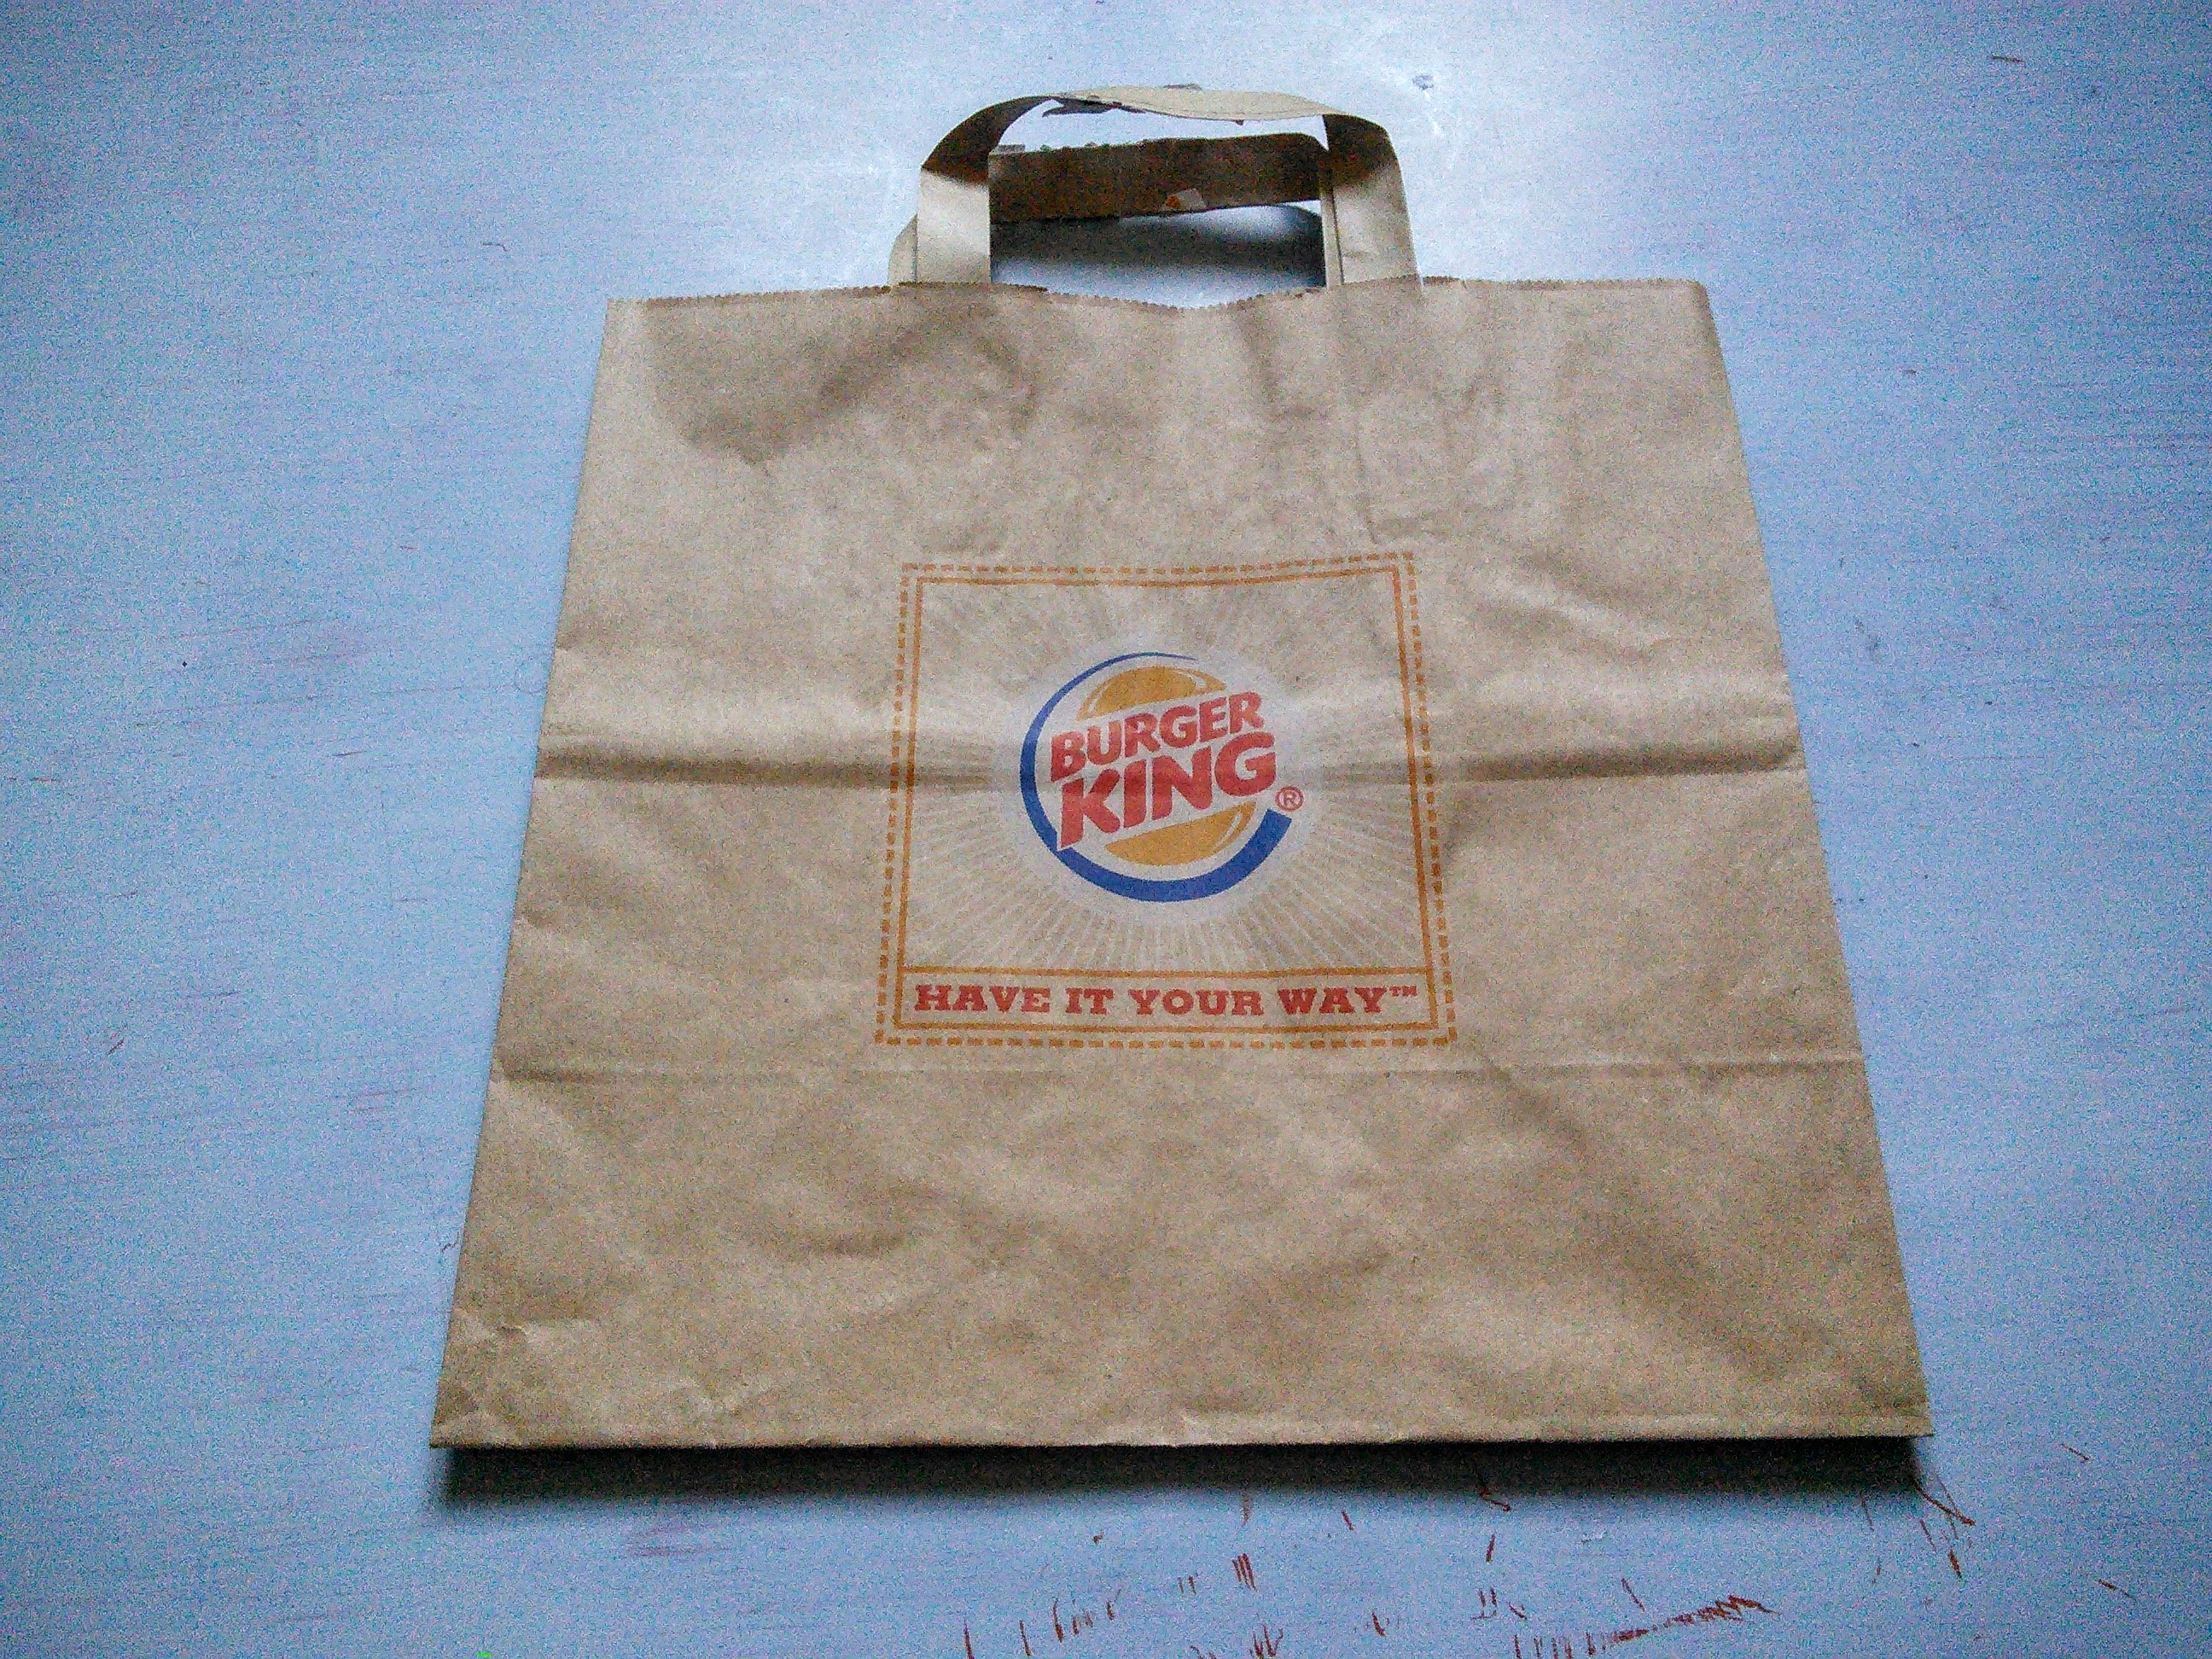
\includegraphics[width=\textwidth]{project_graphics/collected1.jpg}
    \end{subfigure}
    \begin{subfigure}[t]{0.47\textwidth}
        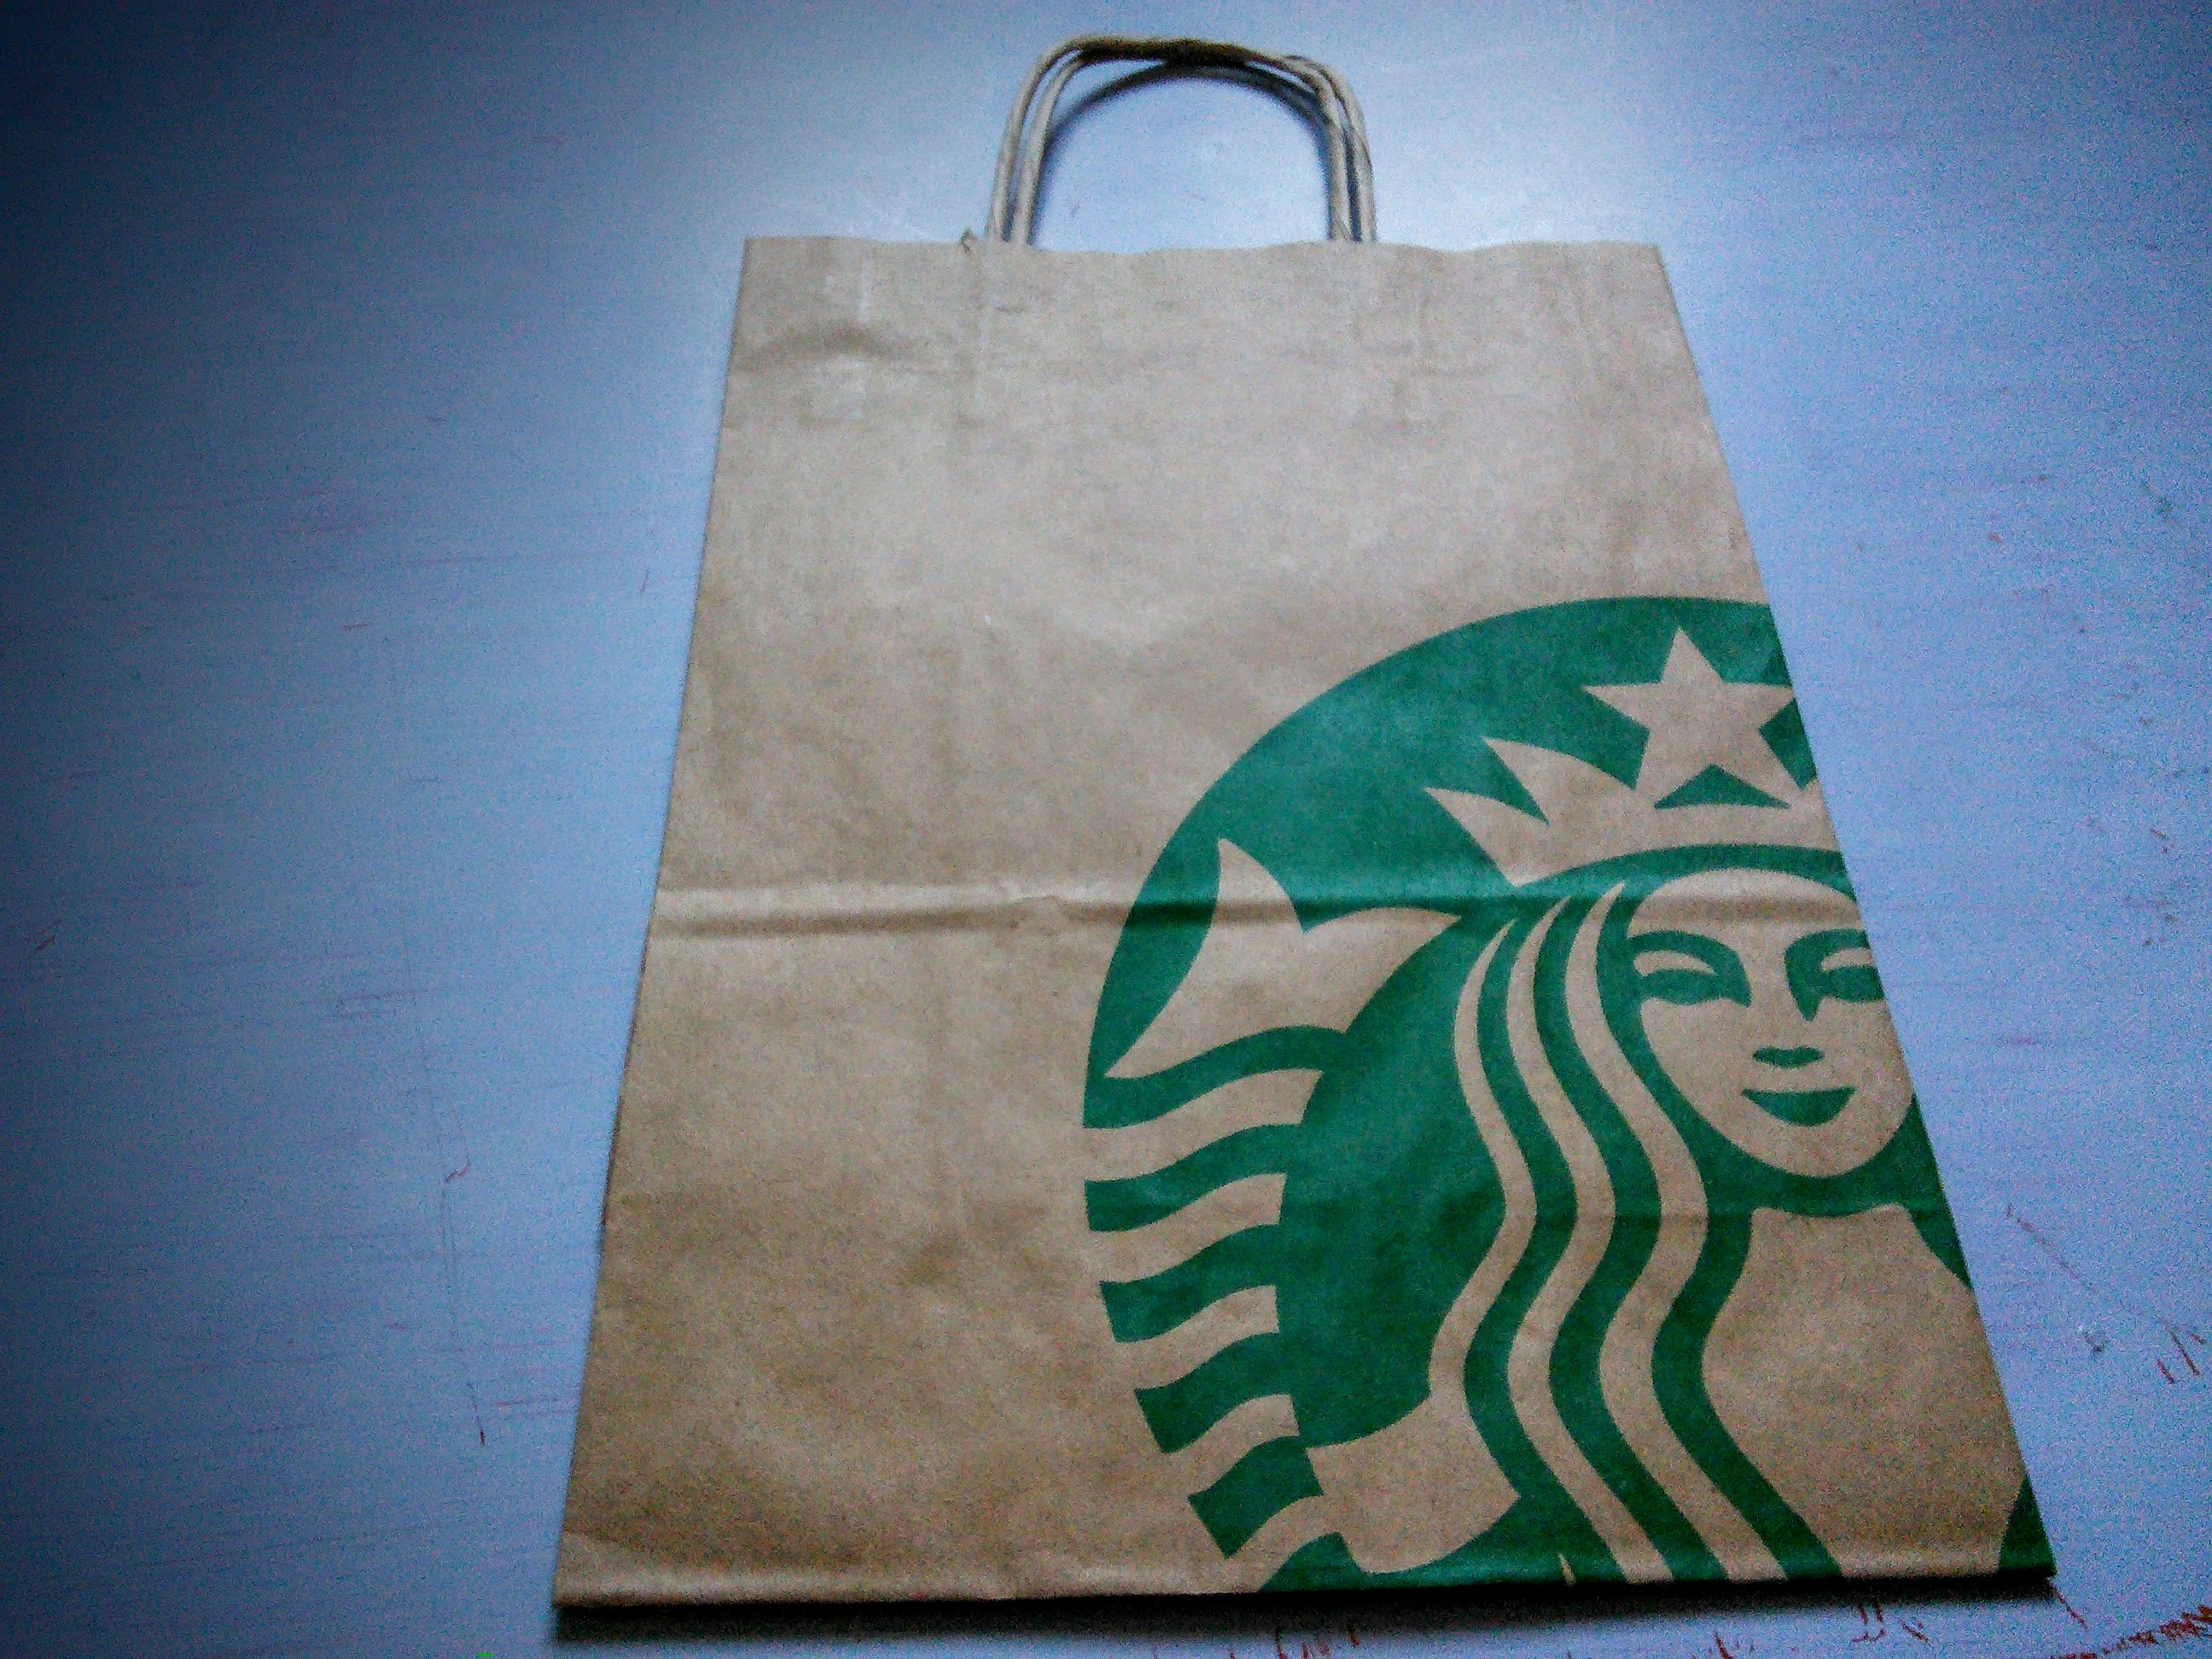
\includegraphics[width=\textwidth]{project_graphics/collected2.jpg}
    \end{subfigure}
    \label{fig:CollectedMaterials1}
\end{figure}